\documentclass[submission,copyright,creativecommons]{eptcs}
\providecommand{\event}{ICLP 2022} % Name of the event you are submitting to
\usepackage{breakurl}             % Not needed if you use pdflatex only.
\usepackage{underscore}           % Only needed if you use pdflatex.
\usepackage{amsmath}
\usepackage{amssymb}
\usepackage{xspace}
\usepackage{listings}
\usepackage[inline]{enumitem}
\usepackage[small]{caption}
\usepackage{subcaption}
\usepackage{booktabs}
\usepackage{graphicx}



\newcommand{\jss}{MPF-JSS\xspace}
\title{Solving a Multi-resource Partial-ordering Flexible Variant of the Job-shop Scheduling Problem with Hybrid ASP}
\author{Giulia Francescutto
\institute{Siemens AG {\"O}sterreich\\ Vienna, Austria}
\email{giulia.francescutto@siemens.com}
\and
Konstantin Schekotihin
\institute{Univeristy of Klagenfurt\\
Klagenfurt, Austria}
\email{konstantin.schekotihin@aau.at}
\and
Mohammed M. S. El-Kholany
\institute{Univeristy of Klagenfurt\\ Klagenfurt, Austria}
\institute{Cairo University\\ Cairo, Egypt.}
\email{mohammed.el-kholany@aau.at}
}
%}
\def\titlerunning{Solving MPF-JSS Problem with Hybrid ASP}
\def\authorrunning{G. Francescutto, K. Schekotihin \& M. El-Kholany}
\begin{document}
\maketitle

\begin{abstract}
  In many industrial environments, scheduling represents a tricky challenge that, if not efficiently dealt with, can prevent a system to be competitive and successful. Scarce resources need to be handled in an effective way, so that the tasks are completed minimizing the waste of time and money. In this work, we propose a \emph{Multi-resource Partial-ordering Flexible Job-shop Scheduling} (\jss) formulation, to capture scheduling scenarios where partially-ordered sequences of operations must be scheduled on multiple required resources, such as tools and specialists.%Scheduling is one of the most complicated problems in manufacturing systems where many tasks should be assigned to the scarce resources while optimizing a particular objective, such as finishing all the tasks as fast as possible or minimizing the delay. The scheduling problem gets complicated when the number of interacting entities increases. Therefore, efficiently controlling these aspects requires a system that can deal with all those features. This work proposes a model that schedules operations by considering multiple required resources such as tools and specialists. 
  The resources are flexible and can process one or more operations based on their characteristics. We have built a model using Answer Set Programming (ASP) in which the execution time of operations is determined using Difference Logic. Furthermore, we introduced two multi-shot strategies that identify the time bounds and find a schedule while minimizing the total tardiness. We conducted experiments on a set of instances provided by a semiconductor manufacturer and the results showed that the proposed model could find schedules for 87 out of 91 real-world instances.
\end{abstract}

\section{Introduction}
Scheduling systems play an essential role in the success/failure of manufacturing industries. An inefficient management of the huge amount of resources that industries dispose of, results in costly delays and waste of expensive machinery. The Job-shop Scheduling (JSS) \cite{johnson1954optimal} problem is one of the most well-known scheduling problems, in which a set of machines should execute a set of jobs represented as a sequence of operations. The goal is to complete all the jobs as soon as possible. From this generic formulation, several other scheduling problems have been defined, by adding extensions with targeted features that have the goal to formalize in the best possible way real-world scheduling scenarios (\cite{brucker1990job} \cite{DBLP:journals/4or/Bellenguez-Morineau08} \cite{DBLP:journals/eor/Dauzere-PeresRL98}). %Flexible JSS extends the classical (JSS) problem where an operation can be performed by many machines. The flexible JSS is more complicated because the machine to execute an operation should be determined and then decide the sequence of the operations assigned to each machine \cite{brucker1990job}. 
%Increasing the number of resources to operate makes the problem harder where in some plants, machines and engineers are required to execute operations. 

In this work, we present the novel Multi-resource Partial-ordering Flexible JSS (MPF-JSS) problem, where multiple resources are needed for executing operations, and jobs require partial-ordered sets of operations to be completed. %Informally, we are given a set of jobs, where each job is described as a partial ordered sequence of operations. We consider two sets of resources that are needed to perform operations. This can be imagined as a scenario where an operation requires both an engineer and a particular machine in order to be executed. Moreover, for each operation, there is more than one resource per resource type that can execute it. 
The goal is to find the best possible allocation of operations to resource wrt. to some predefined criteria, like the minimization of the tardiness. 

To solve MPF-JSS, an encoding using Answer Set Programming with Difference Logic \cite{gebser2016theory} and Multi-shot solving \cite{gebser2019multi} is proposed. Difference constraints allow one to express timing requirements compactly, avoiding grounding issues that occur when a feasible schedule requires a larger time point. We make use of Multi-shot solving to implement two strategies to identify an upper bound on the schedule.
% in which a given set of jobs, represented as a partially-ordered set of operations, and two sets of resources that can perform many operations. These resources are tools and engineers trained to operate these operations while optimizing a particular criterion such as tardiness. |This work introduces a model based on Answer Set Programming with Difference Logic \cite{gebser2016theory} to provide an efficient schedule for solving MPF-JSS problem. We suggested applying two different strategies based on the multi-shot solving technique \cite{gebser2019multi} which allows identifying an upper bound on the schedule. 
We tested our proposed model based on a dataset representing ten working days of an Infineon Fault Analysis lab. The experimental evaluation confirmed that approaching /jss without relying on Multi-shot capabilities is not feasible, when the number of entities involved is significant.  %Each instance represents a whole operational day that was split into smaller instances enabling a detailed assessment of the solving performance. The results showed that obtaining a complete schedule while solving the whole problem in a single shot is impossible. However, applying the multi-shot solving techniques could find schedules for 87 instances out of 91. 

\section{Modeling MPF-JSS with Hybrid ASP}\label{sec:aspmodeling}
We consider a scheduling problem in which different resources are interrelated to process the incoming jobs. In particular, MPF-JSS is an extension of the classical JSS problem where three new aspects are considered: (i) Multi-resources - there are two different resources potentially required to execute an operation; (ii) Partially-ordered- some operations cannot be executed before completing their predecessors and others do not require such constraint; and (iii) Flexible- an operation can be executed by various resources. 
%More specifically, the MPF-JSS is defined as a set of $n$ jobs. Each job has a set of $o$ operations. Some of these operations depend on their predecessors. A set of $m$ machines and $w$ engineers are required to process these operations. The following constraints must be respected:
%\begin{itemize}
%  \item Once the operation starts, it cannot be interrupted.
%  \item Each resource can perform only one operation at a time.
%  \item Operations must be scheduled according to the given partial order.
%  \item The required resources must be available while executing an operation.
%\end{itemize}

Answer Set Programming modulo Difference Logic has been already used in the literature to solve scheduling problems and to overcome the grounding issue occuring when dealing with a large number of possible time points (\cite{DBLP:conf/lpnmr/AbelsJOSTW19}). Here, we also exploit the power of multi-shot solving to find an upper bound on the tardiness and thus provide a good starting point for the optimization methods of an ASP solver. 

We propose two different strategies. The idea of the first approach is to incrementally increase the upper bound on the tardiness of each job in order to identify an interval for which a schedule exists.
%
That is, the algorithm starts by considering the $0$ tardiness bound, and if this yields unsatisfiability (UNSAT), it starts to increment the tardiness bounds by a constant. The parameter values are set via a Python control script, which shifts them by the considered window size in each iteration. 

\begin{figure}[b]
	\centering
	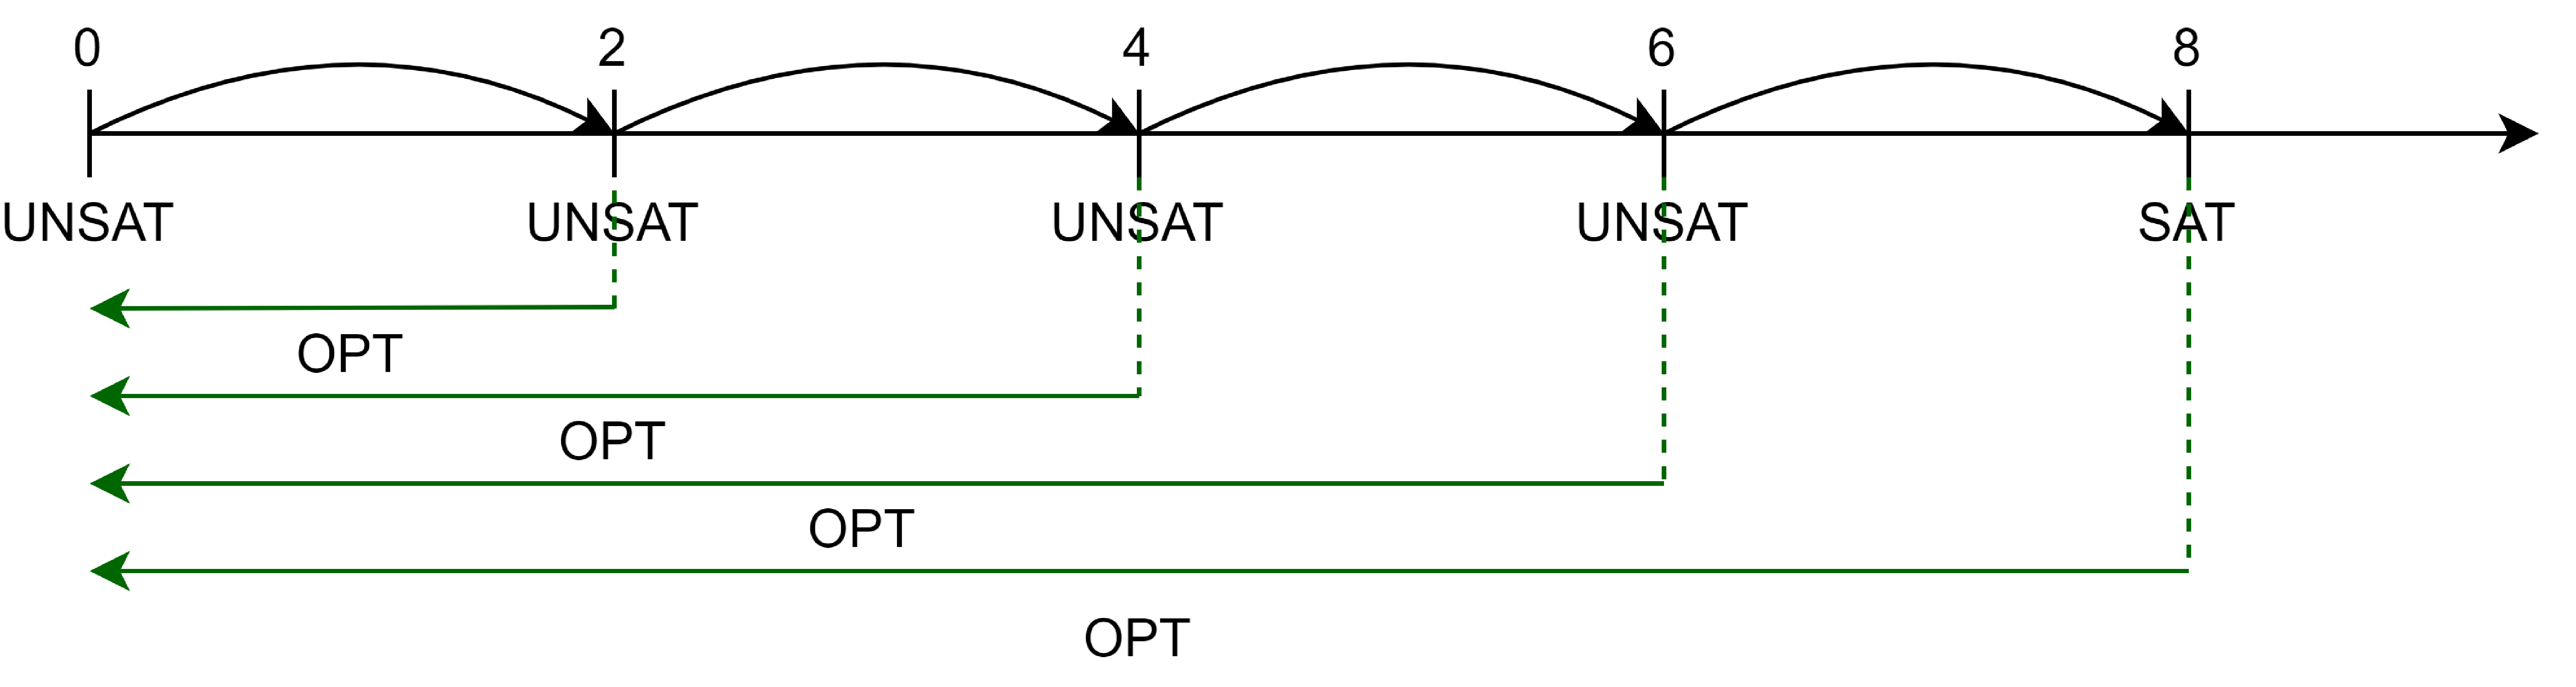
\includegraphics[width=0.5\linewidth]{figures/incremental.pdf}
	\caption{Incremental approach \label{fig:inc}}
        \smallskip %	\vspace{5pt}
        \bigskip
	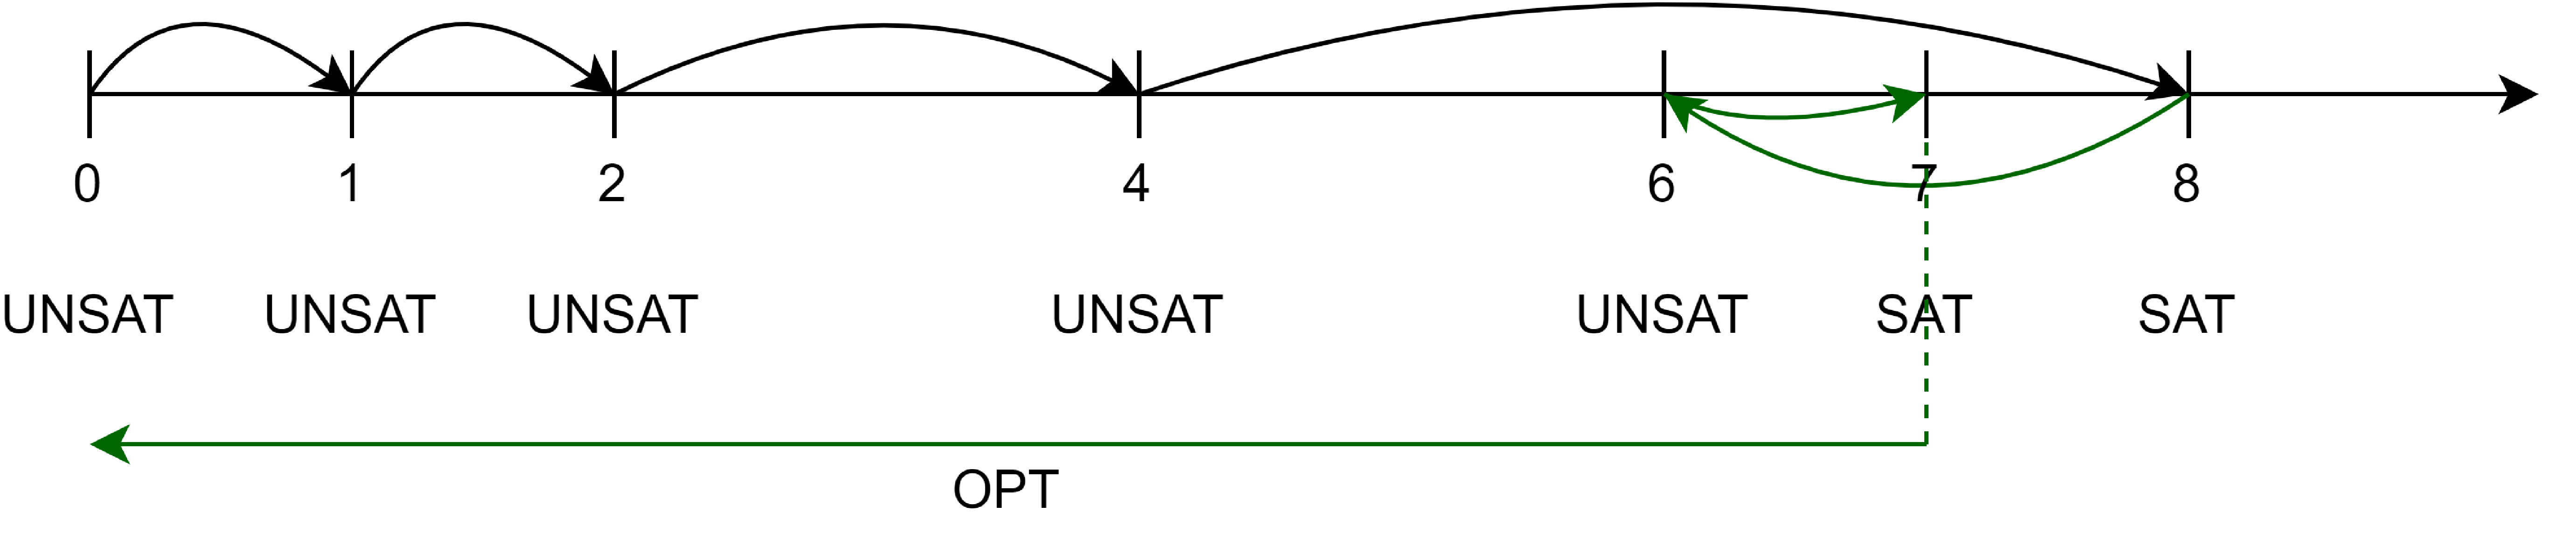
\includegraphics[width=0.5\linewidth]{figures/exponential.pdf}
	\caption{Exponential approach \label{fig:exp}}
\end{figure}

Figure \ref{fig:inc} illustrates a sample execution of the incremental search algorithm, where a tumbling window of size $2$ is moved in each iteration until the target interval for which a schedule exists is found. 

Once the admissible upper bound \lstinline{n} (and a corresponding lower bound \lstinline{m}) is identified, ASP optimization methods search for an optimal solution within this interval.

In the second approach, an upper tardiness bound \lstinline{n} is found by performing a binary search that exponentially increments \lstinline{n} until the first schedule is found, and then converges to the smallest \lstinline{n} for which the scheduling problem is still satisfiable (SAT).

Figure \ref{fig:exp} illustrates the process converging to the upper bound~$7$,
relative to which the tardiness optimization is performed in the second step.

\section{Results}

We conduct our experiments on a set of real-world instances of the \jss problem retrieved from the daily operations history of a semiconductor Fault Analysis (FA) Lab.%  

%We extracted instances for ten random days representing a snapshot of the situation in the lab. The resulting instances have the following approximate number of fixed components defined by the properties of the studied lab:
%\begin{enumerate*}[label=\emph{(\roman*)}]
%	\item $50$ operations,
%	\item $75$ machines, and 
%	\item $45$ workers.
%\end{enumerate*}
%For each of the days chosen the number of open jobs ranges between $30$ and $50$. We split each day-instance into sub-instances, with the aim of having instances of increasing size in multiples of $5$, which resulted into a total of $91$ instances.
We selected ten random days, out of which we extracted instances representing snapshots of the working situation of the lab. We obtained a total of $91$ instances with increasing number of jobs for each day, having the following fixed components:
\begin{enumerate*}[label=\emph{(\roman*)}]
	\item $50$ operations,
	\item $75$ machines, and 
	\item $45$ workers.
\end{enumerate*}
For each obtained instance, we ran three ASP programs: 
\begin{enumerate*}[label=\emph{(\roman*)}]	
	\item \emph{single-shot} -- base program with a tardiness bound precomputed using a heuristic,
	\item \emph{inc} -- the incremental multi-shot ASP variant, and 
	\item \emph{exp} -- the exponential multi-shot ASP search approach.
\end{enumerate*}
%We compared the multi-shot approaches to a single-shot version where the bound is computed in advance as the sum of durations of all operations in an instance.
%This bound is introduced as a constant in the ASP single-shot program.
The experiments were conducted on a workstation with Ubuntu $18.05$, Intel  $3930$K and $64$GB RAM. In our experiments, we use \emph{clingo}[DL] 1.1.0 and \emph{clingo} 5.4.0 with multi-shot solving controlled by the main routine in Python 3.8.5. For each instance, we let the solver run up to a timeout of $2$ hours. For the incremental approach, we chose to use a constant tumbling window of $20$ minutes.

%\begin{figure}[b]
%	\centering
	
%	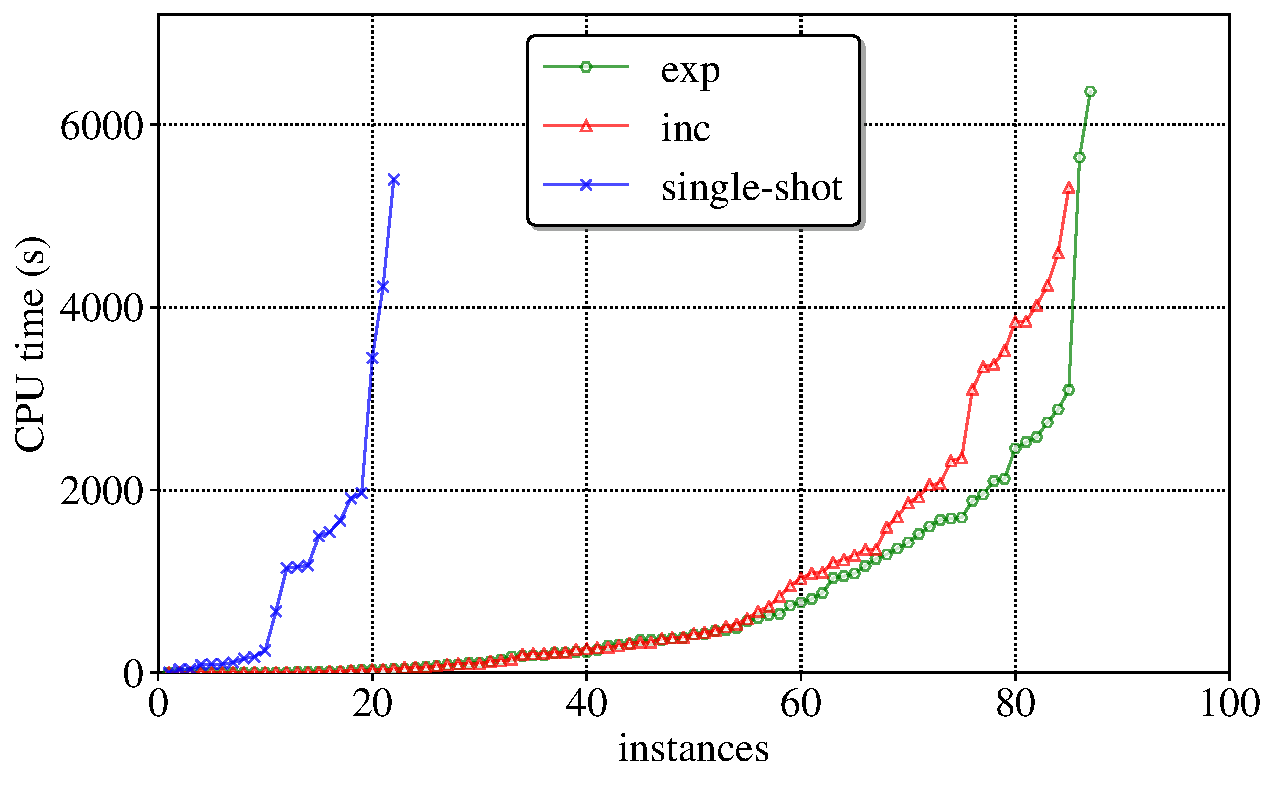
\includegraphics[width=0.75\linewidth]{figures/cactus_time_font20.pdf}
%	\caption{Cactus plot of solving times \label{fig:cactus:time}}
	  
%\end{figure}

%Figure \ref{fig:cactus:time} shows a comparison of the solving performance of the two multi-shot approaches and the single-shot version. %The single-shot program reached the timeout for instances with more than $20$ jobs and only managed to find a schedule for instances with $15$ jobs for two days -- Day 2 and Day 9.
%
The two multi-shot approaches significantly outperformed the single-shot version, that reached the timeout for all the instances having more than $20$ jobs. The exponential version solved $87$ instances out of $91$ within the timeout considered, while the incremental version managed to solve $85$ instances. The exponential approach performs slightly better since it was always finding a tighter upper bound for tardiness, thus, leaving fewer choices for the optimization strategy of the ASP solver. Nevertheless, the differences between the approaches discussed in Section \ref{sec:aspmodeling} were also confirmed in the evaluation. That is, in our experiments, the incremental variant was able to obtain better solutions for three instances with an average total tardiness improvement of 80 minutes.

%\nocite{*}
\bibliographystyle{eptcs}
\bibliography{generic}
\end{document}
